
\documentclass[12pt, a4paper]{article}

\usepackage{graphicx}
\usepackage[utf8]{inputenc}

%Tarih Ekleme
\usepackage[ddmmyyyy]{datetime}
\renewcommand{\dateseparator}{.}
\graphicspath{ {./} }

\usepackage[turkish]{babel}
\renewcommand{\refname}{Kaynaça}
\usepackage{biblatex}

\usepackage{enumitem}
\usepackage{pdflscape}



\addbibresource{kaynakca.bib}



%opening
\title{Virus Vigilante}
\author{Mustafa Akbaba}

\begin{document}
	\begin{figure}
	   		
	   		\centering
	   		
		   	\includegraphics{logo-1.jpg}
	   	\end{figure}




\maketitle





\section{Giriş}
İnternetin hızla gelişmesiyle birlikte kötü amaçlı yazılımlar günümüzde en büyük  siber tehditlerden biri haline geldi.Bilgi çalma, casusluk vb. dahil olmak üzere kötü amaçlı eylemler gerçekleştiren herhangi bir yazılım, kötü amaçlı yazılım olarak adlandırılabilir. \\
Kötü amaçlı yazılımların çeşitliliği artarken, anti-virüs tarayıcıları koruma ihtiyaçlarını karşılayamamakta ve milyonlarca ana bilgisayarın saldırıya uğramasına neden olmaktadır. Kaspersky Labs'a (2023) göre\cite{kasper}, 2023'te Kaspersky'nin sistemleri toplamda yaklaşık 125 milyon zararlı dosya tespit etti. Windows, siber saldırılar için birincil hedef olmaya devam etti ve günlük olarak tespit edilen tüm kötü amaçlı yazılım dolu verilerin yüzde 88'ini oluşturdu. Çeşitli komut dosyaları ve farklı belge formatları aracılığıyla yayılan kötü amaçlı dosyalar, günlük olarak tespit edilen tüm kötü amaçlı dosyaların yüzde 10'unu oluşturarak ilk üç tehdit arasında yer aldı.


\subsection{Proje Nedir?}
	Bu proje makine öğrenimi algoritmalarını kullanarak malware tespiti konusunda  bir çözüm geliştirmektedir. Proje kapsamında, geniş bir  veri seti üzerinde eğitilen bir model ile zararlı yazılım tespitini gerçekleştirecek ve bu alanda yapay zeka tabanlı çözümlerin sağladığı avantajları göstermeye odaklanacak.
\subsection{Projenin Amacı}
Daha önce de belirtildiği gibi, imzalara dayalı kötü amaçlı yazılım dedektörleri, bazı anti-virüs sağlayıcıları tarafından daha önce keşfedilmiş olan ve önceden bilinen kötü amaçlı yazılımlarda iyi performans gösterebilir. Ancak, imzalarını değiştirme yeteneğine sahip polimorfik kötü amaçlı yazılımları ve henüz imzaları oluşturulmamış yeni kötü amaçlı yazılımları tespit edemez. Buna karşılık, anti-virüs uygulamalarının doğruluğu her zaman yeterli değildir, bu da çok sayıda yanlış  ile sonuçlanır\cite{bas}. Yeni tespit yöntemlerinde duyulan ihtiyaç, polimorfik virüslerin yayılma yeteneği ve yayılma oranı ile belirlenmesidir.

\section{Literatür Araştırması}
Sınıflandırma Algoritması kullanımında Machine Learning approach for Malware Detection(2016) projesinden yardım alınmıştır .\cite{git1}Bu yaklaşım, sonuçlarını karşılaştırarak tahmin için hangisinin kullanılacağına karar vermeden önce 6 farklı sınıflandırma algoritmasını dener.
\\
Yapay zekayı kod içinde nasıl kullanılıacağını anlamak için Malware Detection by Machine Learning and Deep Learning(2021) projesinden yardım  alınmıştır.\cite{ytp1}Bu çalışmada kötü amaçlı yazlım tespiti için machine learning ve deep learning yöntemleri kullanılmıştır.
 \\
 Android Malware Detection Using Machine Learning(2022) projesinde konuyu daha iyi kavramak açısından incelemek için kullanılmıştır.\cite{git2}Bu projede, Android kötü amaçlı yazılım tespit sorununu çözmeye yönelik farklı yaklaşımlar sunulmakta ve gösterilmektedir.Bu, makine öğrenimi modelleri aracılığıyla elde edilir. En Önemli Makine Öğrenimi algoritmaları andorid haritalama veri kümelerine uygulanır ve ardından android uygulamasının kötü amaçlı yazılım içerip içermediğini tespit etmemizi sağlar.
 



\section{Metodoloji}
Kötü amaçlı yazılım tespit teknikleri imza tabanlı ve davranış tabanlı yöntemler olarak ikiye ayrılır. Bu yöntemlere geçmeden önce, kötü amaçlı yazılım analizi için kullanılan yaklaşımının temellerini anlamak önemlidir: statik ve dinamik kötü amaçlı yazılım analizi. Adından da anlaşılacağı üzere, statik analiz "statik olarak", yani dosya yürütülmeden gerçekleştirilir. Buna karşılık, dinamik analiz, dosya yürütülürken, örneğin sanal makinede  gerçekleştirilir.
\begin{enumerate}
\item İmza Tabanlı Kötü Amaçlı Yazılım Tespiti
Kötü amaçlı yazılımları tanımlamak için virüs kodlarını/hash'lerini kullanır. Kötü amaçlı yazılım, onu tanımlamak için kullanılan benzersiz bir kod taşır. Bir dosya bilgisayara ulaştığında, kötü amaçlı yazılım tarayıcısı kodu toplar ve bulut tabanlı bir veritabanına gönderir. Veritabanı geniş bir virüs kodu koleksiyonuna sahiptir. Dosya kodu listede bulunursa, veritabanı dosyanın kötü amaçlı yazılım olduğuna dair bir karar verir. Anti-malware dosyayı bilgisayardan reddeder ve siler. Yeni bir kötü amaçlı yazılım keşfedilirse, kodu listeye eklenir.
,,
\begin{itemize}
\item Artıları:
 Bu analizi yöntemi, internette yayılan popüler olan kötü amaçlı yazılım türleri söz konusu olduğunda en hızlı ve en doğru yöntemdir.
\item Eksileri:
Popüler olmayan kötü amaçlı yazılımlar söz konusu olduğunda en doğru yöntem değildir. Doğruluğu kullandığı veri setine bağlıdır.
\end{itemize}
\item Davranış Temelli Kötü Amaçlı Yazılım Tespiti
Kötü amaçlı yazılımları davranışa dayalı olarak tanımlayarak adının hakkını verir. Kötü amaçlı yazılımlar genellikle yasal yazılımlardan farklı davranır. Kötü amaçlı yazılım kendini çalıştırmadan önce bile antivirüs ürünlerine kimliğini açıklayabilecek davranışlar sergileyebilir. Davranış tabanlı tespit, bir yazılımın kötü amaçlı olup olmadığını belirlemek için bu davranışların taranmasını içerir\cite{met1}.
\begin{itemize}
\item Artıları:
Popüler olmayan kötü amaçlı yazılımlar için en iyi sonucu verir.
\item Eksileri:
Taramaya gerek kalmadan mümkün olan en kısa sürede kaldırılması gereken kötü amaçlı yazılımları durdurma yeteneğinden yoksundur.
\end{itemize}
\end{enumerate}
\subsection{Sistem Tasarımı}
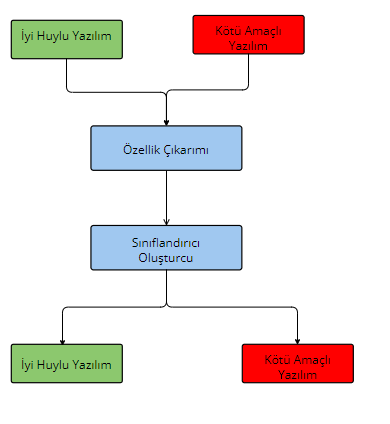
\includegraphics{a.jpg}

\section{Veri Tabanı ve Veriler}
\subsection{Veri Seti}
Başlangıç olarak Kaggle dan alınan Malware\cite{kaggle} adlı veri seti kullanılacak.Projenin ilerlemesine bağlı olarak daha geniş ve daha iyi etiketlenmiş bri veri seti kullanılabilir
\subsection{Kütüphaneler}
Kullanılacak Kütüphaneler:
\begin{itemize}
\item sklearn
\item pyfiglet
\item pefile
\item joblib
\end{itemize}



     


\printbibliography

	


\end{document}


}
